\documentclass[a4paper,11pt]{scrartcl}
\usepackage[utf8]{inputenc}
\usepackage[spanish]{babel}
\usepackage{url}
\usepackage{hyperref}
\usepackage{biblatex}
\usepackage{graphicx}
\graphicspath{ {./img/} }
\addbibresource{references.bib}

%opening
\title{Realidad Aumentada}
\subtitle{Trabajo teórico de la asignatura Interacción Persona-Ordenador 1}
\author{Piotr Maliszewski\\Maciej Nalepa}
\setlength{\parindent}{5ex}


\begin{document}

\maketitle

\begin{abstract}

Esta actividad consiste en la realización de un trabajo teórico sobre interacción avanzada y
nuevos paradigmas de interacción. Para ello el alumno deberá investigar sobre las nuevas
formas de Interacción Persona-Ordenador que están apareciendo en los últimos años, y elaborar un
informe sobre dicha temática, indicando un posible dominio de aplicación, proponiendo y
describiendo un posible escenario de uso.

\end{abstract}

% Introducción y definición de conceptos de la temática seleccionada
\section{Introducción y definición de conceptos}
\subsection{¿Qué es Realidad Aumentada?}
La realidad aumentada es una tecnología que permite combinar los elementos virtuales con el entorno real y representarlos a tiempo real. Gracias a esta tecnología podemos aportar conocimiento al entorno que nos rodea. Para poder entender bien lo que realmente significa realidad aumentada hay que diferenciar desde un principio lo que es la realidad así como la realidad virtual. La definición de la realidad parece más simple de lo que es. Se define el término realidad como todo aquello que existe en el mundo real; mientras que la realidad es aquel entorno que se genera de manera digital y que nos da la sensación de estar inmerso en él.

\subsection{Realidad Virtual y Mixta}
A menudo se puede oír varias nociones como: realidad virtual, realidad aumentada y incluso realidad mixta. Sin embargo esto no es lo mismo. Primero de nada, la realidad virtual construye un mundo nuevo en el que nos sumergimos, mientras que, en la realidad aumentada objetos virtuales parecen aparecer en nuestro propio entorno. En otras palabras la realidad virtual crea un entorno cual podemos percibir en varias maneras y nosotros, es decir nuestros cuerpos no somos la parte coherente del sistema creado. La realidad aumentada aparece alrededor de nosotros. No percibimos todo el entorno artificial, sino déjanos experimentar objetos generados en nuestra vida.
\par La realidad mixta es la más nueva tecnología de las dichas y intenta fusionar las ventajas de sus predecesores. La cosa que diferencia la realidad mixta de la realidad aumentada es que los elementos virtuales interactúan directamente con el entorno. No solo aparecen alrededor, pero también pueden detectar obstáculos y ajustar sus comportamientos a esos. Una grande parte de esta tecnología depende de la realidad aumentada porque está basada en ella.
% [?...] 

\begin{figure}[h]
    \centering
    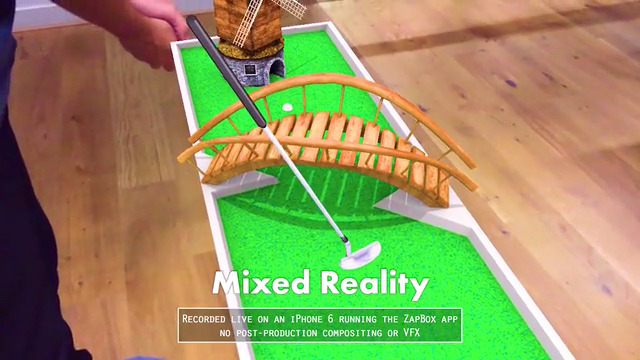
\includegraphics[width=0.7\linewidth]{mixedgolf}
    \caption{Zapbox demo realidad mixta \cite{imgmixedgolf}}
\end{figure}

% Qué indica el Hardware
\subsection{Hardware}
Según Edgar Mozas Fenoll \cite{hardware}, lo que necesita la realidad aumentada para poder colocar los objectos virtuales son siquientes elementos -
Cámara cual capta la imagen del mundo real. El procesador cual debe set capaz de sobreponer los elementos generados por la imagen. Pantalla así que un dispositivo donde se puede mostrar la imagen generada. A menudo la conexión a Internet para recuperar la información asociada con lo que se superpone. Activador así que un objecto real que la realidad virtual reconoce. Eso puede ser un código QR, un marcador, un señal GPS, u al final una imagen o todo un objecto real. La última cosa es un marcador que debe reproducir las imágenes y ser encajado de crearlas en lugares propios.
%

% Estado actual del tema y algunos desarrollos o aplicaciones de interés
\section{Estado actual del tema}
\subsection{Rango de uso actual}
Mucha gente oyó por primera vez de esta tecnología gracias al impacto del juego Pókemon Go \cite{pokemongo}. Los juegos son un gran mercado y aunque a alguien no le gusta la expansión de este mercado, no se puede negar que el mercado de juegos nos permite desarrollar esto. Sin embargo esta tecnología no nos deja solo diversificar nuestro ocio, pero también desarrollar el deporte, la medicina, el marketing, la ingeniería, la educación y muchas otras cosas. Cada año más empresas utilizan la realidad aumentada para hacer el trabajo más eficaz, cómodo y rentable. Afortunadamente no solo los empleados pueden alegrar de esta tecnología. También la gente ordinaria.

\subsection{Capacitar a los trabajadores}
La empresa Lowe's es un buen ejemplo del uso actual de esta tecnología. Lowe's es una compañía minorista donde el servicio al cliente es muy vigente. Hablar con una persona real es la parte de nuestra naturaleza humana. Por esto es importante que la capacitación de agentes de servicio sea sólida. Personal de servicio cual vende una amplia gama de productos debe ser capaz de explicar todo que se ofrece. Para que el entrenamiento sea más rápido, la empresa usa la realidad aumentada\cite{lowe} para habilitar a los trabajadores el acceso a los productos sin la necesidad de manejarlos físicamente. La compañía no solo usa esta tecnología para capacitar su personal, sino que ofrece a los clientes los modelos de alta fidelidad para ver y experimentar las características de los productos antes comprarlos.

\subsection{Reducción de los incertidumbres}
Si  una gran empresa de compras en línea, es posible que tenga un problema. A pesar de lo que comprar en línea se beneficia mucho a la gente, también tiene sus desventajas. No se puede examinar físicamente el producto y por esto más gente devuelve productos comprados en línea que los comprados en las tiendas físicas\cite{seo}. Ikea decidió resolver este problema introduciendo una aplicación moderna\cite{ikea} cual permite disminuir los incertidumbres entre los clientes. Dicha aplicación da la impresión completa permitiendo a los clientes probar los muebles en sus hogares. Esta solución no solo deja a Ikea reducir los costes, sino también ahorra el estrés e las molestias antes de unas compra.

\begin{figure}[h]
    \centering
    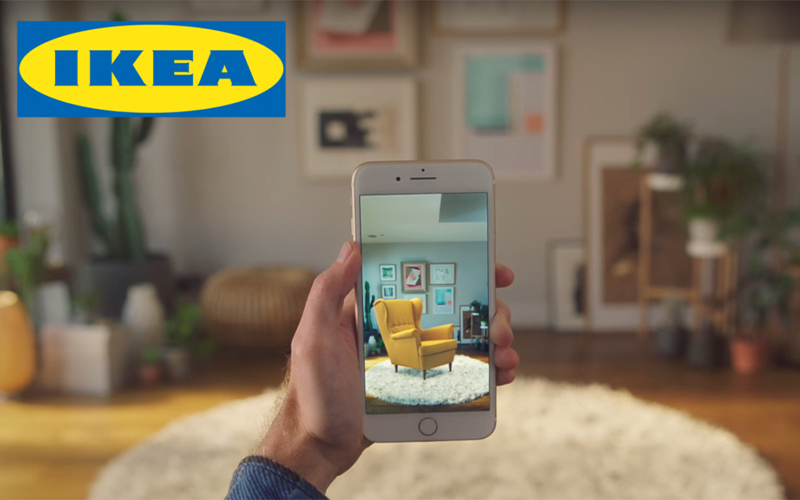
\includegraphics[width=0.7\linewidth]{mixedmarketingikea}
    \caption{IKEA marketing aumentado \cite{imgmixedmarketingikea}}
\end{figure}

\subsection{L'Oréal y Gap}
Otro ejemplo del beneficio de clientes es lo que binda L'Oréal en sus páginas web\cite{loreal}. Los clientes pueden aprovechar esta funcionalidad para probar el producto en directo. Solo se necesita escoger el producto y hacer clic cual abrirá la cámara de dispositivo del usuario. La compañía también ofrece a los usuarios maquillarse de manera virtual y ver como quedaría un tinte antes de adquilerlo.

\par Compañía de ropa Gap lanzó la aplicación\cite{gap} que admite elegir el vestido que interesa al usuario, poner el tamaño y ver como la prenda parecería en vivo de todos lados.

\subsection{Envases interactivas}
Un otro interesante ejemplo de la penetración de la realidad aumentada en nuestra cotidianidad es lo que realiza la compañía Heinz\cite{heinz} con sus publicidades. Los clientes pueden orientar sus teléfonos hasta el producto y ver las receptas. La vista de la comida puede estimular a la compra. La oferta se muestra como un libro en el producto. Esa posibilidad fue introducido ya en 2011 año. Esto demuestra bien que esta tecnología es cerca de nosotros por muchos años.

\subsection{Bindar soporte de autoservicio}
Aun para las empresas uso de la realidad aumentada es rentable no solo antes de compra, sino también ofrecer e tes servicios mientras utilización del producto comprado. Muchas empresas crean un software que soporte autoservicio. Al apuntar un teléfono al coche, los clientes pueden obtener la lista de preguntas frecuentes. Así es como ahorran su tiempo y las empresas tendrán menos consultas porque más usuarios podrán resolver sus problemas independiente.

\par Mercedes implementó un software\cite{mercedes} de asistente virtual Ask Mercedes, a través cual los conductores pueden escanear un componente de su vehículo y comprender la funcionalidad, así como hacer preguntas sobre cualquier problema.

\par Hyundai incluso fue a un paso más allá. En 2015 año, Hyundai lanzó un manual basado en la realidad aumentada\cite{hyundai}. Esto permitió a los conductores usar sus smartphones para obtener el manual. Así pueden no tienen que ver todas las funcionalidades en las páginas, sino verlo a través de sus dispositivos exacto en sus vehículos.
%https://www.la.mercedes-benz.com/es/passengercars/being-an-owner/ask-mercedes-campaign/stage.module.html

%https://news.hyundaimotorgroup.com/MediaCenter/News/Press-Releases/hmc-virtual-guide-introduce-owner-manual-151111

\subsection{Pokémon Go}
La realidad aumentada estaba atrayendo el interés hace unos años gracias al éxito del juego Pokémon Go. En año 2016, cuando fue creado, fue descargado más que 500 millones veces en todo el mundo. Este juego animó a muchas personas a ir afuera para jugar. El juego coloca los pokémones en la ubicación especifico. Utilizando el GPS del móvil, el jugador puede encontrarlos. Sin embargo el juego no haría sucedido si no se hubiera podido ver las entidades. La compañía Niantic implementó la realidad aumentada pare que los objetos no parezcan solo en la pantalla de los móviles, sino para que a través de dispositivo se aparezcan en el mundo real. La aplicación usa el giroscopio y la cámara para mostrar todo. Varios tipos de pokémones aparecían en lugares donde se los esperaba. Por ejemplo los tipos de agua aparecían al lado de los cuerpos de agua. La realidad aumentada creó un nuevo modo de pasar nuestro ocio. En lugar de sentarse al lado del ordenador, más gente salía afuera. Esto animaba más gente a pasar su tiempo más sano y activo.

\begin{figure}[h]
    \centering
    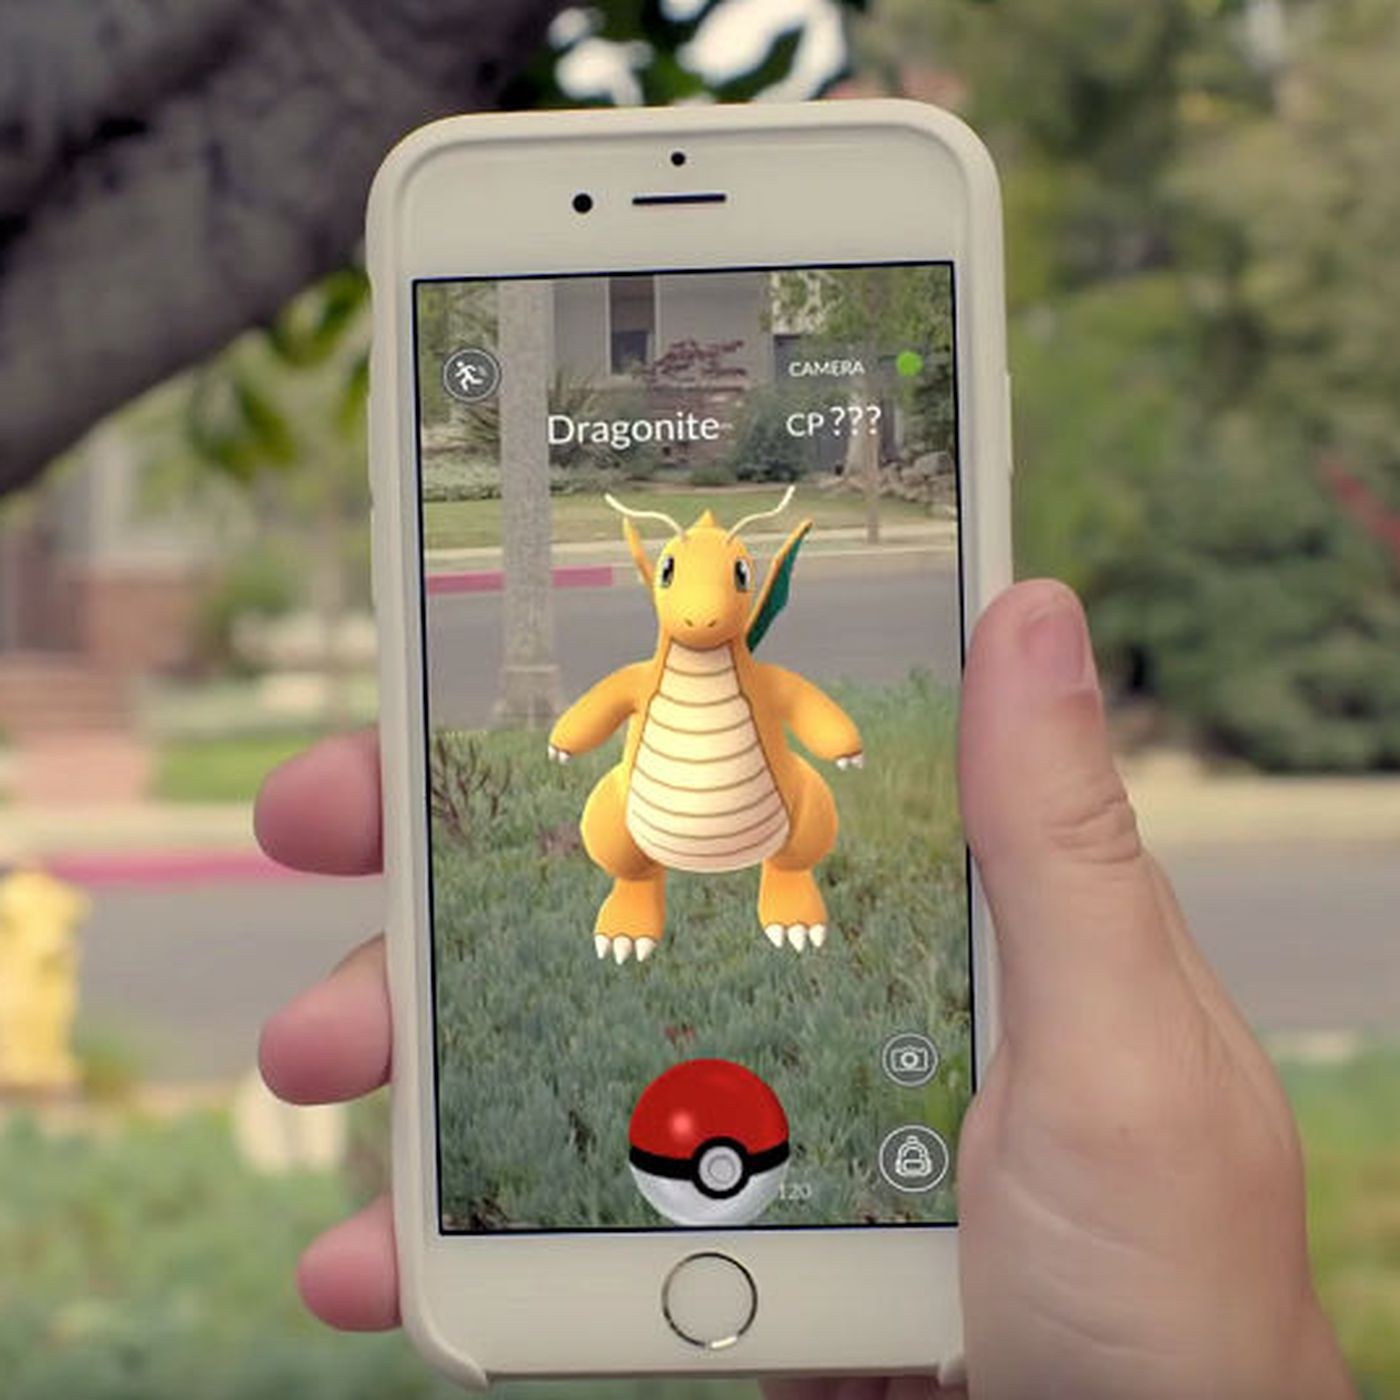
\includegraphics[width=0.5\linewidth]{pokemongo}
    \caption{Pókemon Go \cite{imgpokemongo}}
\end{figure}

\subsection{Turismo}
Un buen ejemplo de usar la realidad aumentada en turismo sería la aplicación Guideo\cite{guideo} que ofrece mostrarte las personajes históricas o mitólogicas también como escenas tradicionales. Para hacer la experiencia más interesante la aplicación binda las imágenes, los vídeos y textos sobre un dado lugar. Gracias a geolicazar tu localización, la aplicación puede presentar te varios recorridos paseos en lugar en que el usuario se encuentra. Después de la descarga la aplicación puede funcionar sin acceso a Internet. Entonces uno que necesitas es un punto Wifiq para disfrutar de las posibilidades.

%%%Todo de los dispositivo: https://www.onirix.com/es/aprende-sobre-ra/hardware-mas-destacado-de-realidad-aumentada-en-2019/
%TODO encontrar los fuentes mejores
\subsection{Microsoft Hololens}
Hololens de Microsoft\cite{hololens} es un producto que usa la tecnología altamente desarrollada. Las gafas usan fibra óptica para mostrar los objetos en los lentes transparentes.
Esta solución permite experimentar el ambiente virtual más que usar verlo mediante la pantalla.
Para que los objetos estén colocados en los sitios dependientes de los lugares reales, las gafas usan varios sensores. Usan ellos también micrófonos que permite dar ordenes para manejar con las gafas. Sensores así como la cámara permiten a usuario controlarlas y un programa en ejecución en varios modos. Hololens detectan tanto la voz como los gestos y los movimientos de ojos y la cabeza. Porque Hololens es capaz a generar los objetos 3D así como interactuar con ellos, se puede usarlo para modificar los modeles en tiempo real. Una ventaja de este dispositivo es lo que no hay que tener llevar más que estas gafas.

%idea: Magic Leap One

\subsection{Epson Moverio}
Esta dispositivo es muy ligero y admite ajustarse a cualquier tamaño, por esto las gafas son muy versátiles. Lo que causa que este producto es aun más versátil es lo que funciona con Android. Por esto facilita el desarrollo de aplicaciones.Está diseñado para empleados y por esto  la imagen es de alta calidad y nítido para hacer más cómodo ver lo que está mostrando en cada condiciones.
Una funcionalidad interesante es lo que, entre otras cosas, gracias a la calidad permite a los usuarios controlar un dron en primera persona con un mando de distancia.

\subsection{Google Glass Enterprise}
 Una de las idea detrás de este producto fue librar las manos de trabajadores. Por esto, para librárselos, el dispositivo permite a usurario controlarse con voz. Todo esto sirve para facilitar el trabajo y eliminar las distracciones. También, de acuerdo de este pensamiento, Google Glass admite a los usuarios a ver los manuales mientras de trabajar para que no se distraan. Las gafas fueron creadas para trabajadores físicos. por esto la batería puede durar mucho y el dipositvo es muy ligero.

%\subsection{Software }
%Algunos de los software de realidad aumentada son:ARToolKit, ATOMIC Web Authoring Tool, Blender, Unity, AR-Media, HP-Reveal, UNREAL ENGINE
%Para desarollar esta tecnología se utiliza varios softwares.

%\subsubsection{}
% Dominio de aplicación elegido y descripción de un posible escenario de uso (se podrán describir los requisitos hardware y software, arquitectura, ...)
\section{Dominio de aplicación y posibles escenarios de uso} 
\subsection{Asistencia}
La aplicación principal de la realidad aumentada es la presentación y la distribución de las informaciones en el entorno del usuario. Por ejemplo, un asistente en una tienda puede buscar y leer las informaciones sobre los productos específicos, como la disponibilidad, en tiempo real y usando gafas. Mecánicos y cirujanos también pueden aprovechar ésta tecnología como ayuda cual extiende las informaciones así como sea una parte de realidad. Para ilustrarlo, imagina una lista de tareas para hacer con el coche, cambiar neumáticos, filtros y aceite. Cada tarea puede ser marcada con un color o descripción y puede ser distinta entre un montón de coches en el taller. Generalmente en cada escenario en cual no se puede ver alguna información posiblemente útil, se puede aplicar la realidad aumentada para ampliar la experiencia en un modo nuevo y más cómodo.

\begin{figure}[h]
    \centering
    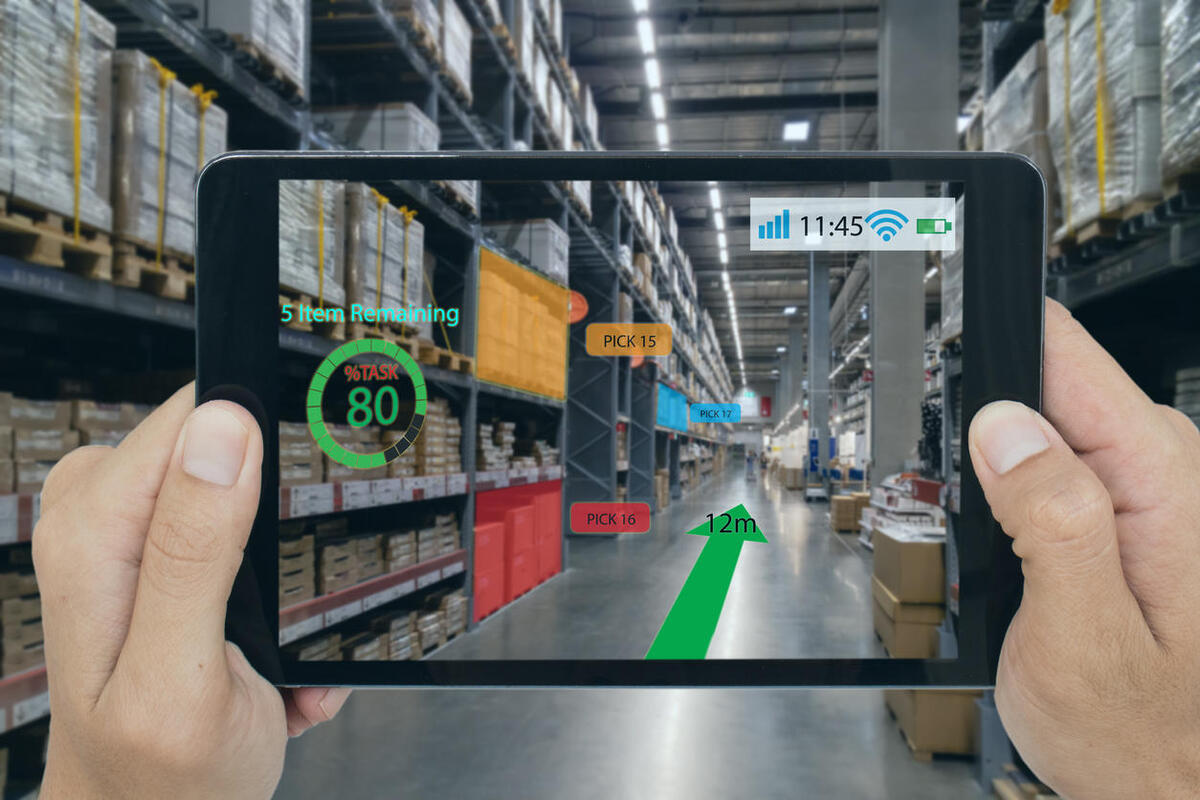
\includegraphics[width=0.7\linewidth]{businessassist}
    \caption{Asistencia comercial \cite{imgbusinessassist}}
\end{figure}

\subsection{Medicina}
El salud es algo que es importante para nosotros todos Desgraciadamente esto es el campo de ciencia cual es extremadamente difícil para enseñar. En la medicina, hay que pasar muchísimas horas aprendiendo sobre el cuerpo humano. Si los modeles realísticos fueran disponibles a la gama de personas más amplia, la sociedad tendría los expertos mejor educados, con los modeles más parecidos a los reales y además los estudiantes de medicina no tendrían que pasar tanto tiempo estudiando como curar la gente. La realidad aumentada podría dejarlos tener más oportunidades para ver los órganos tan como parecen en la realidad. También sería posible simular la operación para que lo puedan experimentar solos. Sin embargo, no solo con la enseñanza nos puede soportar esta tecnología. Se lo dejará a médicos obtener la información sobre el estado actual de un paciente a través de las gafas ligeras cuales no le van a molestar a un médico durante su trabajo. Haciendo los rayos X, le permite al médico superponer algo de la imagen de un dispositivo al cuerpo del paciente. Gracias a esto, ubicar los sitios donde habrá que operar o tomar otras medidas.
 
\subsection{Educación}
La educación es vigentísima, y con el paso de los años se hace incluso más importante. La educación nos lleva varios beneficios. Es inconcebiblemente duro imaginarse nuestro mundo sin todos los especialistas. El mundo sigue haciéndose mejor gracias a los todos que desarrollan, inventar y idean siguientes invenciones, proyectos e teoremas. Los medios de enseñanza cuales puede ofrecer la realidad aumentada, podrían en futuro asegurar mejores resultados. No solo en la mencionada medicina, en la educación más alta se puede mejorar el rendimiento del aprendizaje. Mostrar varias imágenes a los niños, puede interesarlos más con varios temas. Gracias a esa solución la educación infantil podría ser más efectiva. Los modelos 3D de los planetas o de los átomos y las moléculas dejará a los alumnos experimentar e entender lo que están estudiando. La visualización será un siguiente paso de desarrollar la educación antes, imprimir los libros era una revolución. Luego el progreso de la digitalización y difundir los ordenadores y Internet dejó a multitud de gente aprender más que normalmente habrían podido. Todo eso es la posibilidad cual podemos aprovechar por un bienestar de las próximas generaciones.
 
\subsection{Turismo}
Ya ahora hay aplicaciones cuales pueden enriquecer nuestras experiencias mientras viajar. Sin embargo los soluciones cuales se utiliza no son tan avanzadas. Mejorar los modeles y detectar del mundo puede llevar más sensaciones en el sector del turismo. En los museos de la historia natural la gente podrá ver a los viejos animales en movimiento alrededor de ellos. La arma, los trajes de varias épocas y maquinas de los viejos años podrán ver también. Pero el uso de esa tecnología no se limita solo a los modeles de museos. Los caminos históricos en las ciudades se podrán generarse también. Los turista serán capaz de ir a lo largo de varias posibles rutas y ver no solo las reconstrucciones de los edificios, sino también la gente de la propia época en los lugares con monumentos. Para la gente corriente, será posible descubrir los lugares interesantes así como leer sobre la historia mientras se observa los monumentos a través de un visualizador.
 
 
\begin{figure}[h]
    \centering
    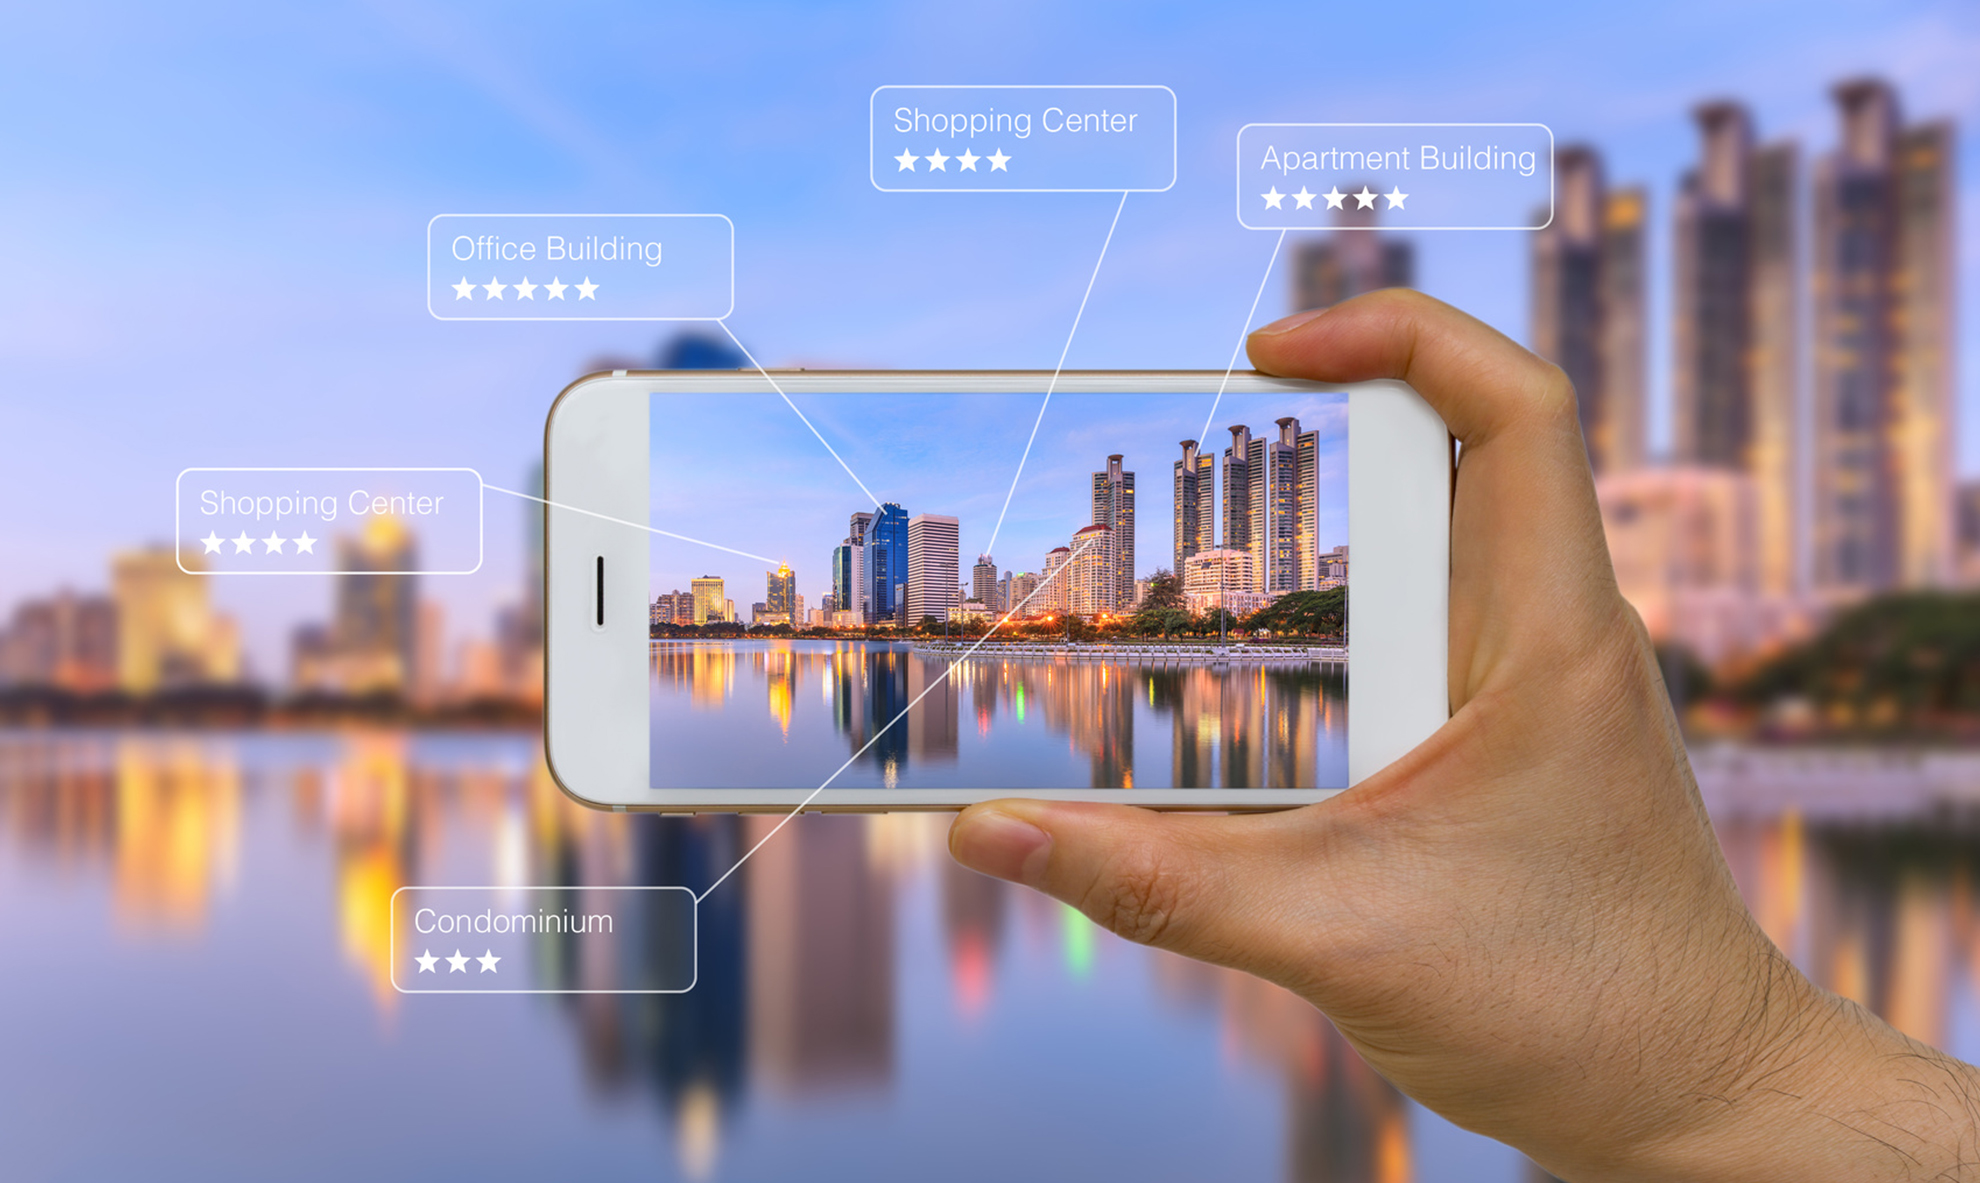
\includegraphics[width=0.7\linewidth]{augmented}
    \caption{La realidad aumentada en turismo \cite{imgaugmented}}
\end{figure}
 
\subsection{Navegación}
La realidad aumentada ya es utilizada para navegar. Sin embargo no se navega a los conductores de los coches, sino los pilotes de caza. Los aviones de casa ya utilizan sistemas complejos. El futuro puede traernos una solución parecida para los coches y incluso más complejo. En el parabrisas un programa podría mostrar a un conductor las flechas de la dirección de conducción, la información del coche y de la situación en la carretera. Todo en relación de un conductor para su conveniencia. Hoy en día echar un vistazo a la navegación y no mirar a la carretera expone a un accidente. Así que además de la conveniencia esta tecnología garantiza la seguridad.

\begin{figure}[h]
    \centering
    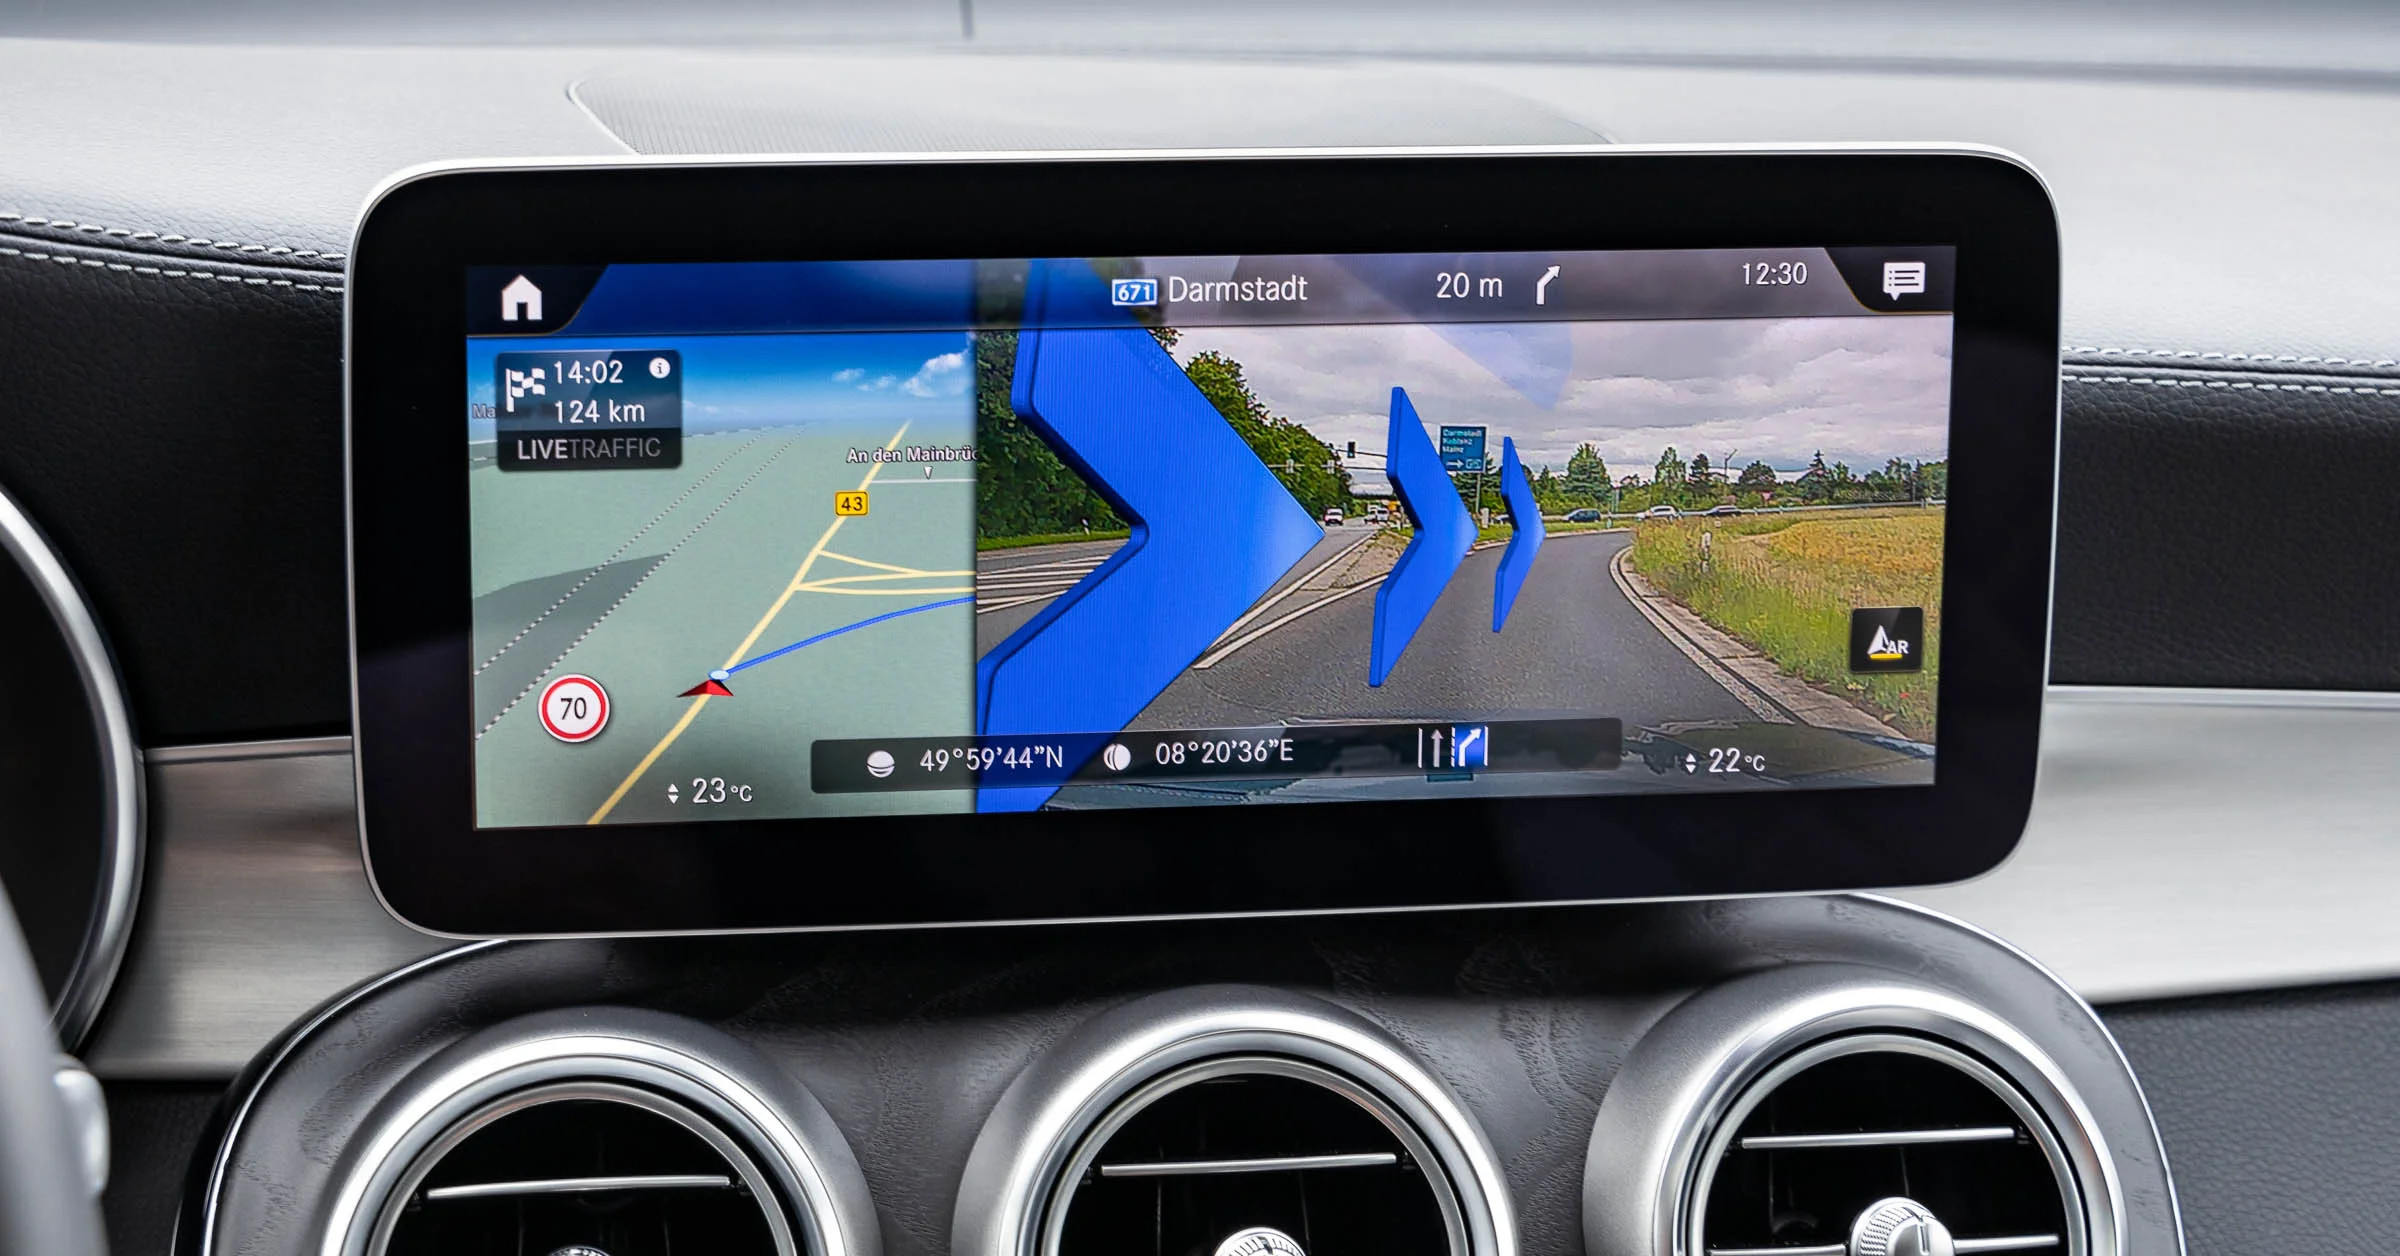
\includegraphics[width=0.7\linewidth]{mercedesnavigation}
    \caption{Mercedes navegación aumentada \cite{imgmercedesnavigation}}
\end{figure}
 
%\subsection{Dispositivo personal}
 
% Conclusiones y opinión personal
\section{Conclusiones}
En resumen, la realidad aumentada es una evolución de interfaces, cual nos permite usar nuestro entorno como una estructura de la interfaz. El desarrollo de la realidad aumentada está consiguiendo con mejoramiento de nuestros teléfonos móviles porque eso es una forma más accesible a la gente. Varios dispositivos mejoran la experiencia del usuario más sino todavía están muy carros y impopulares. A pesar de esto el futuro de la realidad aumentada es brillante porque nos permita aplicar la interfaz de nuestro dispositivo en cualquier lugar e en modos creativos.

% Referencias bibliográficas consultadas
\section{Referencias}
\printbibliography
\end{document}
